\documentclass[11pt]{article}

% Pacotes
\RequirePackage{luatex85}
\usepackage{amsmath}
\usepackage{amssymb}
\usepackage{graphicx}
\usepackage[colorlinks=true, allcolors=blue]{hyperref}
\usepackage{amsthm}
\usepackage{framed, color,xcolor}
\usepackage{stmaryrd}
\usepackage{rotating}           % Usado para rotacionar o texto
\usepackage[all,knot,arc,import,poly]{xy}   % Pacote para desenhos gráficos
% Este pacote pode conflitar com outros pacotes gráficos como o ``pictex''
% Então é necessário usar apenas um dos pacotes conflitantes
\usepackage{tikz, tikz-cd}
\usepackage{epigraph}
\usetikzlibrary{babel}
\usetikzlibrary{positioning}
\usetikzlibrary{calc}
\usepackage[stix2]{newtxmath}
\usepackage{mathtools, nccmath}
%\usepackage[usenames,dvipsnames]{xcolor}
\usepackage{amssymb, mathrsfs}
\usepackage[numbers]{natbib}
\usepackage{fontspec}
\usepackage{enumitem} % pra substituir o símbolo do itemize por alguma coisa legal, tipo setinhas:  \begin{itemize}[label=\ding{212}]
\usepackage{pifont}
\usepackage{stmaryrd} % for \arrownot (notação de adjacência em grafo)
\usepackage{quiver} %pacote do quiver pra desenhar diagramas mais legais

%Fontes e Línguas
\usepackage[portuguese]{babel}
%\usepackage{eufrak}
\usepackage{emoji}
\setmainfont{DarwinSerif-Regular.otf}
\newfontfamily\fakebold[FakeBold=1.75]{DarwinSerif-Regular.otf}
\newfontfamily\fakeitalic[FakeSlant=0.2]{DarwinSerif-Regular.otf}
\renewcommand{\textbf}[1]{{\fakebold#1}}
\renewcommand{\textit}[1]{{\fakeitalic#1}}
\renewcommand{\bfseries}{\fakebold}
\renewcommand{\itshape}{\fakeitalic}



%Cores


%Comandinhos que gosto
\usepackage{mathtools}
\newcommand{\defeq}{\vcentcolon=}
\newcommand{\eqdef}{=\vcentcolon}
\newcommand{\bigslant}[2]{{\raisebox{.2em}{$#1$}\left/\raisebox{-.2em}{$#2$}\right.}}
\newcommand{\logo}{\Rightarrow}
\newcommand{\pulinho}{\vspace{.5cm}}
\newcommand{\edge}{%
  \mathrel{-}% minus as a relation
  \joinrel\joinrel % some backup
  \mathrel{-}% minus as a relation
}
\newcommand{\notedge}{%
  \mathrel{\mkern2mu}% a small advancement
  \arrownot % a short slash
  \mathrel{\mkern-2mu}% compensate
  \edge
}

\newcommand{\Aut}{\text{Aut}}
\newcommand{\Cay}{\text{Cay}}

\newcommand{\luafacil}{
\emoji{waxing-crescent-moon}
}

\newcommand{\luamedio}{
\emoji{first-quarter-moon}
}

\newcommand{\luadificil}{
\emoji{waxing-gibbous-moon}
}

\newcommand{\luaprojeto}{
\emoji{full-moon}
}

\let\varphi\phi

%Caixinhas coloridas

\theoremstyle{definition}
\newtheorem{theorem}{Teorema}
\newenvironment{teorema}{
\definecolor{shadecolor}{HTML}{f59aa3}
\begin{shaded}
\begin{theorem}
}
{
\end{theorem}
\end{shaded}
}

\theoremstyle{definition}
\newtheorem*{theorem*}{Teorema}
\newenvironment{teorema*}{
\definecolor{shadecolor}{HTML}{f59aa3}
\begin{shaded}
\begin{theorem*}
}
{
\end{theorem*}
\end{shaded}
}

\theoremstyle{definition}
\newtheorem{prop}{Proposição}
\newenvironment{proposicao}{
\definecolor{shadecolor}{HTML}{FFDBDF}
\begin{shaded}
\begin{prop}
}
{
\end{prop}
\end{shaded}
}

\theoremstyle{definition}
\newtheorem*{prop*}{Proposição}
\newenvironment{proposicao*}{
\definecolor{shadecolor}{HTML}{FFDBDF}
\begin{shaded}
\begin{prop*}
}
{
\end{prop*}
\end{shaded}
}

\theoremstyle{definition}
\newtheorem{cor}{Corolário}
\newenvironment{corolario}{
\definecolor{shadecolor}{HTML}{f59aa3}
\begin{shaded}
\begin{cor}
}
{
\end{cor}
\end{shaded}
}

\theoremstyle{definition}
\newtheorem*{cor*}{Corolário}
\newenvironment{corolario*}{
\definecolor{shadecolor}{HTML}{f59aa3}
\begin{shaded}
\begin{cor*}
}
{
\end{cor*}
\end{shaded}
}



\theoremstyle{definition}
\newtheorem{definition}{Definição}
\newenvironment{definicao}{
\definecolor{shadecolor}{HTML}{defcfc}
\begin{shaded}
\begin{definition}
}
{
\end{definition}
\end{shaded}
}

\theoremstyle{definition}
\newtheorem*{definition*}{Definição}
\newenvironment{definicao*}{
\definecolor{shadecolor}{HTML}{defcfc}
\begin{shaded}
\begin{definition*}
}
{
\end{definition*}
\end{shaded}
}

\theoremstyle{definition}
\newtheorem{example}{Exemplo}
\newenvironment{exemplo}{
\definecolor{shadecolor}{HTML}{b9e6d3}
\begin{shaded}
\begin{example}
}
{
\end{example}
\end{shaded}
}

\theoremstyle{definition}
\newtheorem*{example*}{Exemplo}
\newenvironment{exemplo*}{
\definecolor{shadecolor}{HTML}{b9e6d3}
\begin{shaded}
\begin{example*}
}
{
\end{example*}
\end{shaded}
}

\theoremstyle{definition}
\newtheorem{veronica}{Lema}
\newenvironment{lema}{
\definecolor{shadecolor}{HTML}{FFF1F2}
\begin{shaded}
\begin{veronica}
}
{
\end{veronica}
\end{shaded}
}

\theoremstyle{definition}
\newtheorem*{veronica*}{Lema}
\newenvironment{lema*}{
\definecolor{shadecolor}{HTML}{FFF1F2}
\begin{shaded}
\begin{veronica*}
}
{
\end{veronica*}
\end{shaded}
}

\newenvironment{prova}{\paragraph{Demonstração:}}{\hfill$\square$ 
\pulinho
}

\newenvironment{aviso}{
\definecolor{shadecolor}{HTML}{fffe9a}
\begin{shaded}
}{\end{shaded}}

\theoremstyle{definition}
\newtheorem{exersisio}{Exercício}
\newenvironment{exercicio}{
\definecolor{shadecolor}{HTML}{CFB5FF}
\begin{shaded}
\begin{exersisio}
}
{
\end{exersisio}
\end{shaded}
}

%Tamanho do papel
\usepackage[a4paper,top=1cm,bottom=1cm,margin=3.5cm]{geometry}



%%%%%%%%%%%%%%%%%%%%%%%%%%%%%%%%%%%%%%%%%%%%%%%


%Definições só pra esse texto
\usepackage[bb=boondox]{mathalpha}



\title{Se para todos existe um então existe um para todos}
\author{Violeta Mar}
\date{}


\begin{document}

\maketitle

\begin{center}
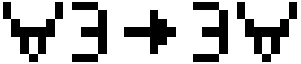
\includegraphics[scale=0.7]{desenhos/good.png}
\end{center}

% ULTRAFILTROS E COMPACTIFICAÇÕES DAS COISAS

% Teorema da compacidade - modelos, Ultrafiltros - F Limite, Tychonov

% versão mais fraca: Konig's lemma, lema de seleção de rado

% Aplicações: 

% análise: análise não standard

% grafos: De Bruijn–Erdős theorem, teoremas de finito pro localmente finito (teorema casamento de hall, teorema de konig e seus amigos)

% poset: Dilworth's theorem

% álgebra: robinson's principle: If a first-order sentence holds in every field of characteristic zero, then there exists a constant p such that the sentence holds for every field of characteristic larger than, ax-grothendieck theorem

% autômatos celulares: garden of eden theorem

% conjuntos: submodelos elementares




% Intuições: 

% -> compacidade é a 'generalização de finito pra infinito' - pra cada `direção pro infinito', coloque um ponto a mais que captura essa direção - isto compactifica seu espaço

% -> quando algo é compacto, suas propriedades gerais são capturadas pelas propriedades de seus subconjuntos finitos


% Proposta de roteiro:

% 1o dia: começar com konig lemma e  de brujin erdos contável. lógica! teorema da compacidade em lógica de primeira ordem. aplicações: upward Lowen-Skolem (modelos elementares pra cima), nonstandard models de PA, completude de ACF e consequências,

% 2o dia: "existencia de ultrafiltro", ultraproduto, prova de compacidade via ultraproduto, nonstandard analysis

% 3o dia: topologia! generalizar konig lema com "limite inverso de não vazio é não vazio", tychonoff, mostrar como o teorema de compacidade pode ser visto nesse framework, aplicação: infinite ramsey implica finite ramsey?


\section{Dia 1}

Vamos tentar descrever um fenômeno que se repete muitas vezes pelo mundo da Combinatória Infinita. Chamamos de `o fenômeno da compacidade', onde, em algum sentido, uma estrutura infinita pode ser construída colando coerentemente estruturas finitas. Existem muitas formulações equivalentes, e em diferentes níveis de força. Vou dar aqui as minhas favoritas, com tentativas de construir intuição sobre como elas funcionam, e me esforçando para minimizar pré-requisitos. Noções gerais de topologia, lógica e conjuntos provavelmente vão ser o suficiente para acompanhar o texto, e se não forem, espero que as referências ajudem - além delas também aprofundarem a discussão.

Ao longo do texto, coloco exercícios para interromper o fluxo de leitura passiva e incentivar uma atividade do leitor (você). Eles são marcados com um nível de dificuldade: \luafacil são mais alongamentos do que exercícios, coletando continhas ou raciocínios rotineiros; \luamedio são realmente exercícios, pedem mais atenção e tempo; \luadificil são desafios para os apaixonados, e \luaprojeto são jornadas, projetos de pesquisa ou problemas em aberto.

Vamos começar com a versão mais simples do fenômeno - o Lema de König. Imagine que você está construindo algo, passo a passo, que vai precisar de um número infinito (enumerável...!) de passos para ser completado. Mas tem um problema: a cada passo, você tem finitas escolhas a serem feitas, e algumas delas podem levar a ruas sem saída, ou seja, passos onde não há escolhas possíveis para se continuar. O Lema de König é uma formulação do fato simples de que, se em todo momento existe uma escolha que leva a infinitas mais escolhas, então existe pelo menos um jeito de se completar a sua construção. Em um desenho:

\begin{center}
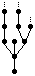
\includegraphics[scale=1.5]{desenhos/konig.png}
\end{center}

Visualizamos cada estado da nossa construção (ou seja, construções parciais) como uma destas bolinhas, e realizar um passo é subir através de uma aresta até outra bolinha acima. O lema será uma afirmação sobre desenhos deste tipo, que chamamos de árvores, formalizadas na linguagem de teoria de grafos.

Rapidinho, as definições necessárias. Um grafo é um conjunto $V$, cujos elementos chamamos de vértices, com uma relação simétrica $E \subset V \times V$, representando quando dois vértices em $V$ estão ligados por uma aresta (neste caso, dizemos que os dois vértices são vizinhos ou adjacentes). Um caminho em um grafo é uma sequência de vértices $(v_n)$ onde existe sempre uma aresta entre $v_n$ e $v_{n+1}$. Um grafo é conexo se dados dois vértices, existe um caminho entre eles. Um grafo é uma árvore se ele é conexo e não contém ciclos, ou seja, caminhos que começam e terminam no mesmo vértice. Um grafo é infinito quando ele possui infinitos vértices, e um caminho é infinito se ele passa por infinitos vértices. Um grafo é localmente finito se todo vértice só está ligado a finitos outros vértices.

Para brincar com as definições:

\begin{exercicio}
  \luamedio Se convença que uma árvore infinita com uma escolha de vértice é a mesma coisa que uma sequência infinita $(T_n)$ de conjuntos com funções $f_n:T_{n+1} \rightarrow T_n$ e $T_0$ contendo apenas um ponto (dica: $T_0$ é o vértice escolhido, $T_{n+1}$ são os vizinhos dos vértices em $T_n$, e $f_n$ te diz como eles estão conectados).

  Nessa formulação, prove que a árvore é localmente finita se e somente se cada $V_n$ é finito.
\end{exercicio}

Esse primeiro exercício não vai ser necessário para a demonstração do lema de König, mas mais tarde vamos usar essa formulação pra generalizar o lema pra uma versão mais forte de compacidade.

\begin{teorema}[Lema de König]
 Uma árvore infinita localmente finita sempre contém um caminho infinito.
\end{teorema}
\begin{prova}
  Vamos começar nosso caminho infinito numa árvore $T$ a partir de um vértice arbitrário $v_0 \in T$. Como $T$ é infinita e conexa, existem infinitos caminhos diferentes partindo de $v_0$. O próximo vértice depois de $v_0$ em um qualquer um destes caminhos é um vértice vizinho de $v_0$. Mas $v_0$ só contém finitos vizinhos, então deve existir pelo menos um vizinho tal que infinitos caminhos partindo de $v_0$ tem como segundo vértice este vizinho. Escolha este vizinho para ser o nosso próximo vértice $v_1$. Agora temos infinitos caminhos saindo de $v_1$ e, lembrando que caminhos não repetem vértices, podemos então repetir o mesmo argumento que acabamos de fazer com os vizinhos de $v_0$ menos o $v_1$. Assim, obtemos outro $v_2$ vizinho de $v_1$ com infinitos caminhos partindo dele. Continuando assim, indutivamente, construímos um caminho infinito $(v_n)$.
\end{prova}

Vamos aplicar este resultado pra provar uma simplificação de um resultado clássico da teoria de grafos infinitos. Colorir vértices é uma grande diversao dos teoristas de grafos: uma $k$-coloração de um grafo é uma associação de cada vértice a uma cor dentre um conjunto de $k$ cores de forma que vértices vizinhos recebem cores diferentes. Uma pergunta simples de se fazer é, dado um grafo, qual o menor número de cores que precisamos ter para conseguirmos fazer uma coloração? Um resultado famoso desta área é o teorema das quatro cores, que diz que se o seu grafo é planar (intuitivamente, isso significa que ele pode ser desenhado em um plano sem arestas cruzando) então com certeza com $4$ cores você consegue. Provar isto é surpreendentemente difícil, e foi uma das primeiras demonstrações feitas com assistência de computadores nos anos 70. Este teorema foi provado pra grafos finitos, mas ele vai valer para infinitos também porque aqui conseguimos usar o truque da compacidade: reduzimos a pergunta da existência de uma $k$-coloração em um grafo infinito para a existência de uma $k$-coloração em cada um dos seus subgrafos finitos (lembrando aqui que um subgrafo é obtido através de um subconjunto de vértices e também um subconjunto de arestas do seu grafo maior).

\begin{teorema}[De Bruijn-Erdös localmente finito]
  Seja $G$ um grafo (infinito) localmente finito. Existe uma $k$-coloração para $G$ se e somente se existe uma $k$-coloração para cada subgrafo finito $G' \subset G$.
\end{teorema}
\begin{prova}
  Vamos chamar $k$-coloração apenas de coloração pra facilitar nossa vida. A ida é clara - uma coloração do grafo todo se reduz a uma coloração de seus subgrafos. Primeiro perceba o problema da volta. Se começarmos a partir de uma coloração qualquer de um subgrafo $G'$, gostaríamos de extender esta coloração. Poderiamos ingenuamente pensar: tome um subgrafo maior contendo $G'$ e tome uma coloração para este subgrafo maior. Mas ela pode não extender a coloração original, ou seja, ela pode escolher cores diferentes das quais você tinha escolhido antes para os vértices de $G'$. Assim, não é claro porque um processo indutivo que iria aumentando os subgrafos considerados e tomando as colorações existentes realmente convergeria para uma coloração bem definida após infinitos passos. Pra isso acontecer, estas colorações precisam estar `encaixadas', ou seja, concordarem umas com as outras. Conseguimos mostrar a existência destas colorações encaixadas através do Lema de König.\\

  Vamos construir uma árvore $T$ indutivamente. Escolha um vértice qualquer de $G$ e considere o subgrafo finito $G_0$ contendo apenas este vértice. Defina $G_{n+1}$ como sendo o subgrafo de $G$ contendo $G_n$ e todos os vizinhos dos vértices de $G_m$. Agora, o primeiro vértice $r$ de $T$ será uma coloração arbitrária de $G_0$, e chamamos $T_0 = \{r\}$ de nível $0$ da árvore. Os próximos vértices serão todas as colorações de $G_1$ que extendem a coloração associada à $r$ e os ligamos com uma aresta ao $r$. Estes vértices coletamos no conjunto $T_1$, que chamamos de nível $1$ da árvore. Indutivamente, se já construímos um nível $T_n$ onde todos os elementos correspondem a colorações de $G_n$, criamos o nível $T_{n+1}$ com um vértice para cada coloração de $G_{n+1}$ e pra cada um destes, o ligamos ao vértice de $T_n$ correspondendo a coloração de $G_n$ da qual ela extende.\\

  Como $G$ é infinito, então $T$ é infinito, e como $G$ é localmente finito, cada um dos $G_n$ vão ser finitos e logo $T$ é localmente finito. Pelo Lema de König, $T$ deve conter um caminho infinito. Um caminho infinito em $T$ corresponde a uma sequência de colorações dos $G_n$, uma extendendo a outra. Logo a união de todas estas colorações é uma coloração bem definida. Esta coloração está definida na união de todos os $G_n$, que é $G$.
\end{prova}

A brincadeira aqui foi usar uma árvore que capturava como construções locais se extendiam (como eles eram coerentes entre si), e o lema de König garantia uma sequência destas construções locais que se extendiam mutuamente, e portanto definiam uma construção global coerente para estrutura toda. A fraqueza do lema de König é que você precisa pedir que existam apenas finitas extensões de cada construção (a hipótese de `localmente finito'). Vamos capturar agora o fenômeno de compacidade na sua versão mais forte - o Teorema da Compacidade da lógica de primeira ordem. Ele vai ser capaz de provar o De Bruijn-Erdös para qualquer grafo, não só os localmente finitos.\\

Vamos fazer um rapidíssimo resumo de o que é a lógica de primeira ordem, focando apenas nas definições necessárias para afirmarmos o Teorema da Compacidade. Recomendo bastante o texto da Anush para quem quiser ver mais detalhes - vou fazer referência a esse texto algumas vezes no livro. \\

A ideia aqui é capturar, em uma linguagem formal, o processo de raciocínio matemático. Os símbolos de uma \textbf{linguagem} de primeira ordem $L$ vão ser

\begin{itemize}[label=\ding{212}]
  \item os conectivos lógicos $\vee,\wedge, \lnot, \rightarrow$
  \item os quantificadores $\exists, \forall$
  \item para cada natural $n$ um símbolo de variável $v_n$
  \item o símbolo de igualdade $=$
  \item um conjunto $R$ de símbolos de relações
  \item um conjunto $F$ de símbolos de funções
  \item um conjunto $C$ de símbolos de constantes
  \item pontuações $, ( )$
\end{itemize}

Para especificarmos $L$, precisamos decidir quantos símbolos de relações, funções e constantes vamos ter, e também qual a `aridade' de cada relação e função (a aridade vai representar quantos `inputs' uma relação ou uma função recebe, quando formos interpretar estes símbolos). Uma \textbf{assinatura} $\sigma$ consiste exatamente disso: um cardinal para cada $R,F$ e $C$ e duas funções $\sigma_R: R \rightarrow \mathbb{N}, \sigma_F: F \rightarrow \mathbb{N}$ que interpretamos como especificando as aridades.

A linguagem $L_{\text{Con}}$ de teoria de conjuntos é a dada pela seguinte assinatura: temos $0$ constantes, $0$ funções e $1$ símbolo relacional, que denotamos como $\in$, que tem aridade $2$.

A linguagem $L_{\text{Grf}}$ de teoria de grafos é dada pela seguinte assinatura: temos $0$ constantes, $0$ funções e $1$ símbolo relacional, que denotamos como $\edge$, que tem aridade $2$.

Espera, mas essas estruturas são iguais! Apenas usamos um nome diferente pro símbolo de relação binária de cada um. O que está acontecendo aqui é simples: em conjuntos nos importamos apenas com uma relação, a de pertencimento, e em grafos, com a de adjacência. As expressões destas linguagem são as mesmas, mas vamos ver grande diferença quando formos considerar a semântica destas expressões. Por exemplo, em teoria de conjuntos, um dos axiomas em essência diz que $\lnot \exists x (x \in x)$ (não existe conjunto que pertence a ele mesmo), mas em teoria de grafos poderia valer que $\exists x (x \edge x)$, já que isso acontece com um grafo que contém um um vértice com uma aresta que liga o vértice nele mesmo.

A linguagem $L_{\text{Grp}}$ de teoria de grupos é dada pela seguinte assinatura: temos $1$ constante, denotada por $e$, temos $1$ função de aridade $2$, denotada por $*$ e $0$ relações.

A linguagem $L_{\text{Art}}$ da aritmética é dada pela seguinte assinatura: temos $1$ constante, denotada por $0$, temos $3$ funções, denotadas por $S$ de aridade $1$ (sucessor), $+$ de aridade $2$ (soma) e $\cdot$ de aridade $2$ (produto) e $0$ relações.

\begin{exercicio}
  \luafacil Dê uma assinatura possível para a teoria de anéis.
\end{exercicio}

Queremos juntar estes símbolos em `frases' (strings) que gostaríamos que expressassem de alguma maneira afirmações sobre objetos matemáticos. Primeiro descrevemos quais são as formas permitidas de se juntar estes símbolos para se criar estas frases (sintática), e depois vamos descrever como decidir o que estas frases estão expressando, isto é, a interpretação com significado delas (semântica). 

Fixe uma linguagem $L$ definida por alguma assinatura $\sigma$. Uma \textbf{expressão} é simplesmente uma sequência arbitrária de símbolos da linguagem (por exemplo, digamos, $\exists \exists ( v f \forall$, uma bagunça). Vamos escolher um subconjunto comportado de expressões. Primeiro definimos \textbf{termos}. Símbolos de variáveis e símbolos de constantes são termos, e se $t_1, \dots, t_n$ são termos e $f$ um símbolo de função com aridade $n$ então a expressão $f(t_1,\dots, t_n)$ é um termo.

\begin{exercicio}
  \luafacil Dê exemplos de termos na linguagem da aritmética.
\end{exercicio}

Com termos, podemos definir \textbf{fórmulas}. Primeiramente, as \textbf{fórmulas atômicas} são expressões da forma

\begin{itemize}[label=\ding{212}]
  \item $t = s$ onde $t,s$ são termos
  \item $r(t_1, \dots, t_n)$ onde $t_1, \dots, t_n$ são termos e $r$ é uma relação de aridade $n$.
\end{itemize}

O conjunto de todas as fórmulas é construido recursivamente a partir das atômicas e de usos sucessivos dos conectivos lógicos e dos quantificadores. Formalmente, uma expressão é uma fórmula se ela é de uma das formas

\begin{itemize}[label=\ding{212}]
  \item \lnot \phi
  \item \phi \vee \psi
  \item \phi \wedge \psi
  \item \phi \rightarrow \psi
  \item \exists v \phi
  \item \forall v \phi
\end{itemize}

para alguma fórmula $\phi$ ou para duas fórmulas $\phi,\psi$, com $v$ sendo algum símbolo de variável.

Os nomes que estamos dando para todos estes símbolos (variáveis, constantes, conectivos lógicos e etc) sugerem fortemente qual é o significado que queremos que as fórmulas tenham. Por exemplo, na linguagem da aritmética, $\forall v (S(v) + v = S(v + v))$ é a afirmação que queremos que diga que para todo número natural $v$, a soma de $v$ com seu sucessor é igual ao sucessor da soma de $v$ com ele mesmo. Formalmente, no entanto, até agora definimos apenas um conjunto especial de strings de símbolos. Para definirmos a semântica, precisamos de algo que vamos chamar de estrutura.\\

Uma \textbf{estrutura} para uma linguagem $L$ é a escolha de:

\begin{itemize}[label=\ding{212}]
  \item um conjunto $M$ (o chamado `universo de discurso')
  \item para cada símbolo de constante $c \in C$, um elemento $c_M \in M$
  \item para cada símbolo de função $f \in F$ com aridade $n$, uma função $f_M: M^n \rightarrow M$
  \item para cada símbolo de relação $r \in R$ com aridade $n$, uma relação $r_M \subset M^n$
\end{itemize}

Agora estamos falando de funções, relações e constantes de verdade, não apenas símbolos!\\

Vamos interpretar as fórmulas em $M$. Pra isso vamos ter que passar pelo rito de passagem levemente sofrido no estudo de lógica de primeira ordem que é falar de variáveis livres e substituições de constantes. Perceba que nas nossas fórmulas, permitimos que símbolos de variáveis não estejam sempre ligados a quantificadores. No exemplo que demos da linguagem da aritmética,a fórmula $\forall v (S(v) + v = S(v + v))$ dizia uma afirmação sobre todos os números mas a expressão $S(v) + v = S(v + v)$ também é uma fórmula - porém aqui, $v$ está `livre' (não quantificado). 

\begin{exercicio}
  \luamedio Dê uma definição formal para quando uma fórmula contém uma variável livre, e defina uma \textbf{sentença} como uma fórmula sem variáveis livres. (se você se embananar, dê uma olhada na definição da Anush)
\end{exercicio}

Dada uma fórmula $\gamma$ com variáveis livres dentre os símbolos $v_1, \dots, v_n$, e uma escolha de $n$ elementos $m_1,\dots, m_n$ em $M$, vamos definir formalmente o que significa que $\gamma$ vale em $M$ com cada $v_i$ substituído pelo $m_i$. Denotamos isto como $M \vDash \gamma[v_1 \rightarrow m_1,\dots, v_n \rightarrow m_n]$. Quando $n = 0$, ou seja, $\gamma$ é sentença, então escrevemos apenas $M \vDash \gamma$. Se você já viu isso antes, ou a definição é muito intuitivamente óbvia para você do que deveria significar, se sinta livre para pular os próximos parágrafos...

Começamos com as fórmulas atômicas. Primeiramente

\begin{exercicio}
  \luafacil Dado uma estrutura $M$, se convença que para cada termo sem variáveis livres $t$ temos um elemento $t_M \in M$. Já para um termo $t$ com $n$ variáveis livres, temos um elemento $t_M[v_1 \rightarrow m_1,\dots, v_n \rightarrow m_n] \in M$ para cada escolha de $n$ elementos $m_1,\dots, m_n$ em $M$.
\end{exercicio} 

Se sua fórmula for da forma $t = s$ para dois termos ou $r(t_1,\dots,t_n)$ para uma relação $r$ e termos $t_1,\dots, t_n$, então diga que

\begin{itemize}[label=\ding{212}]
  \item $M \vDash (t = s) [v_1 \rightarrow m_1,\dots, v_n \rightarrow m_n]$ se vale que $t_M[v_1 \rightarrow m_1,\dots, v_n \rightarrow m_n] = s_M [v_1 \rightarrow m_1,\dots, v_n \rightarrow m_n]$
  \item $M \vDash r(t_1,\dots,t_n)[v_1 \rightarrow m_1,\dots, v_n \rightarrow m_n]$ se vale que $r_M(\tilde{t_1},\dots,\tilde{t_n})$ onde $\tilde{t_i} = (t_i)_M[v_1 \rightarrow m_1,\dots, v_n \rightarrow m_n]$.
\end{itemize}

Notação feia, porém espero que o significado esteja claro. Se a fórmula não é atômica, então, defina recursivamente que

\begin{itemize}[label=\ding{212}]
  \item $M \vDash \lnot \phi[v_1 \rightarrow m_1,\dots, v_n \rightarrow m_n]$ se não vale que  $M \vDash \phi[v_1 \rightarrow m_1,\dots, v_n \rightarrow m_n]$
  \item $M \vDash \phi \vee \psi$ se vale que $M \vDash \phi[v_1 \rightarrow m_1,\dots, v_n \rightarrow m_n]$ ou $M \vDash \psi[v_1 \rightarrow m_1,\dots, v_n \rightarrow m_n]$
  \item $M \vDash \phi \wedge \psi$ se vale que $M \vDash \phi[v_1 \rightarrow m_1,\dots, v_n \rightarrow m_n]$ e $M \vDash \psi[v_1 \rightarrow m_1,\dots, v_n \rightarrow m_n]$
  \item $M \vDash \phi \rightarrow \psi$ se vale que $M \vDash \psi[v_1 \rightarrow m_1,\dots, v_n \rightarrow m_n]$ sempre que $M \vDash \psi[v_1 \rightarrow m_1,\dots, v_n \rightarrow m_n]$
  \item $M \vDash \exists v \phi[v_1 \rightarrow m_1,\dots, v_n \rightarrow m_n]$ se existe um elemento $m \in M$ tal que $M \vDash \phi[v \rightarrow m, v_1 \rightarrow m_1,\dots, v_n \rightarrow m_n]$
  \item $M \vDash \forall v \phi[v_1 \rightarrow m_1,\dots, v_n \rightarrow m_n]$ se pra todo elemento $m \in M$ vale que $M \vDash \phi[v \rightarrow m, v_1 \rightarrow m_1,\dots, v_n \rightarrow m_n]$
\end{itemize}

\begin{exemplo*}
\begin{itemize}[label=\ding{212}]
\item Um grafo $G$ é uma estrutura para a linguagem da teoria de grafos, onde tomamos o universo de discurso como sendo os vértices de $G$ e a relação $\edge$ como sendo a relação de adjacência entre os vértices. Um grafo qualquer satisfaz $G \vDash \forall v \forall w (v \edge w) \rightarrow (w \edge v)$.
\item Uma estrutura pra linguagem da aritmética é o conjunto de números naturais $\mathbb{N}$ como universo de discurso, com $S$ como sendo a função sucessora $x \rightarrow x + 1$, $+$ como sendo a operação de soma e $\cdot$ como sendo a operação produto.
\item Uma estrutura muito esquisita para a linguagem da aritmética seria tomar $M$ como sendo o conjunto dos números inteiros $\mathbb{Z}$, $S$ a função $x \rightarrow 2x$, $+$ a função $ (x,y) \rightarrow x - y$ e $\cdot$ a função $(x,y) \rightarrow x + y$.
\end{itemize}
\end{exemplo*}

Finalmente, podemos então dizer o que é um modelo! Se $T$ é um conjunto de sentenças (fórmulas sem variáveis livres), então uma estrutura $M$ é um modelo deste $T$ se vale que $M \vDash \phi$ pra todo $\phi \in T$. Denotamos isso como $M \vDash T$ e geralmente dizemos que $M$ satisfaz $T$.

\begin{exercicio}
  \luamedio Relembre alguns dos axiomas de ZFC, os escreva na linguagem de teoria de conjuntos, e encontre algum modelo para estes axiomas.
\end{exercicio}
Vamos recompensar o leitor que passou por esse montante de definições técnicas com o enunciado do lindíssimo resultado central do nosso minicurso:

\begin{teorema}[Teorema da Compacidade]
  Seja $T$ um conjunto de sentenças de alguma linguagem de primeira ordem. Existe um modelo para $T$ se e somente se para cada subconjunto finito $T' \subset T$ existe um modelo que satisfaz $T'$.
\end{teorema}

A demonstração clássica desse resultado primeiro passa pelo famoso Teorema de Completude de Gödel (não o de Incompletude!). Completude, em essência, diz que a única obstrução para a existência de um modelo para uma teoria $T$ é a existência de uma prova da contradição a partir de $T$ (em outras palavras, existe modelo para $T$ se e somente se $T$ não prova uma contradição). Aqui precisamos definir a noção de prova, que é onde introduziriamos regras de inferência e axiomática da lógica de primeira ordem. Vamos evitar essa discussão, e trazer uma demonstração puramente semântica do Teorema da Compacidade (através de ultraprodutos) na próxima seção.

\begin{exercicio}
  \luamedio Se já sabe (ou consegue imaginar, ou foi pesquisar) a definição de prova em lógica de primeira ordem, esboce a prova de Compacidade usando Completude. A ideia é simples: provas são finitas!
\end{exercicio}

Vamos finalizar essa primeira parte com a demonstração da versão sem restrições do Teorema de De Bruijn–Erdős.

\begin{teorema}[De Bruijn–Erdős]
    Seja $G$ um grafo (infinito). Existe uma $k$-coloração para $G$ se e somente se existe uma $k$-coloração para cada subgrafo finito $G' \subset G$.
\end{teorema}
\begin{prova}
Tome um grafo infinito $G$. Adicione à linguagem da teoria de grafos uma constante $c_v$ para cada vértice $v$ de $G$. Adicione também, para cada $i$ natural entre $1$ e $k$, uma relação $r_i$ de aridade $1$, que iremos usar para dizer que um vértice está colorido ou não pela cor $i$. Seja $\tilde{L}$ a linguagem resultante. Defina as fórmulas
\begin{itemize}[label=\ding{212}]
  \item $\gamma: \forall x (r_1(x) \vee r_2(x) \dots \vee r_k(x))$ 
  \item $\phi_{ij}: \forall x(r_i(x) \rightarrow \lnot r_j(x))$ para todo $i \neq j$
  \item $\psi_{i}: \forall x \forall y (((x \edge y) \wedge r_i(x) )\rightarrow \lnot r_i(x))$
\end{itemize}
A primeira fórmula diz que todo vértice é dado uma cor, as fórmulas do segundo item dizem que os vértices são dados exatamente uma cor, e as fórmulas do terceiro item dizem que vértices adjacentes recebem cores diferentes. Seja $\phi$ a fórmula gerada pela conjunção ($\wedge$) de todas as fórmulas $\gamma$, $\phi_{ij}$ e $\psi_i$ (isto é possível pois são apenas finitas fórmulas).

Agora, para cada par de vértices $v,w$ de $G$, vale que ou $v \edge w$ ou $\lnot (v \edge w)$. Se vale o primeiro caso, seja $\alpha_{vw}$ a fórmula $c_v \edge c_w$ e o no segundo caso a fórmula $\lnot (c_v \edge c_w)$. Defina $T \defeq \{\alpha_{vw} \mid v,w \in G\} \cup \{\phi\}$.

\begin{exercicio}
  \luafacil Se convença que um modelo para $T$ é exatamente um grafo isomorfo a $G$ com uma $k$-coloração.
\end{exercicio}

Tome um subconjunto finito $T' \subset T$. Se $T'$ não contém $\phi$ então $G$ é um modelo para $T'$. Suponha que $T'$ contém $\phi$. Como $T'$ é finito, só aparecem finitas constantes $c_v$. Considere o subgrafo $G'$ de $G$ com todos os vértices associados às constantes que aparecem em $T'$, junto com todas as arestas entre eles existentes em $G'$. Por hipótese, existe uma $k$-coloração para $G'$. Então $G'$ é um modelo para $T'$. Concluimos pelo Teorema da Compacidade que deve existir um modelo para $T$, ou seja, deve existir uma $k$-coloração para $G$.

\end{prova}

\begin{exercicio}[Modelo Não-Standard para a Aritmética]
  \luadificil Seja $L_{\text{Art}}$ a linguagem da aritmética e $\mathbb{N}$ o conjunto dos números naturais. Seja $T$ o conjunto de todas as fórmulas $\phi$ tal que $\mathbb{N} \vDash \phi$. Use o Teorema da Compacidade para provar que existe um modelo para $T$ não isomorfo ao dos números naturais.

  Um possível caminho: defina recursivamente os termos $t_0 \defeq 0$ e $t_{n+1} \defeq t_n + 1$. Seja $\tilde{L}$ uma extensão de $L_{\text{Art}}$ adicionando apenas uma constante $\omega$. Considere as fórmulas $\phi_n : \omega = t_n$ na linguagem $\tilde{L}$. Seja $\tilde{T} = T \cup \{\phi_n \mid n \in \mathbb{N}\}$. Use Compacidade em $\tilde{T}$ para achar um modelo para $\tilde{T}$, e argumente que este modelo deve ser um modelo para a aritmética não isomorfo ao $\mathbb{N}$.
\end{exercicio}

\section{Dia 2}

Definir ultrafiltro. Provar Lema do Ultrafiltro. 

Exemplos simples: F-Limite.

Fixe uma linguagem $L$ em alguma assinatura. Suponha que temos uma coleção de estruturas $M_i$ indexados por algum conjunto $I$. Seja $u$ um ultrafiltro de $\mathcal{P}(I)$. Considere o produto $\prod_{i \in I} M_i$. Defina a relação de equivalência $(m_i) \sim_u (m'_i)$ se o conjunto $\{i \in I \mid m_i = m'_i\}$ é selecionado por $u$. Repare aqui na nossa notação: quando escrevemos $(m_i)$ isso representa a sequência cujos elementos são $m_i$ para cada $i \in I$ e quando escrevemos $m_i$ sem os parentêses queremos dizer o elemento de $M_i$ que é o $i$-ésimo da sequência $(m_i)$.

\begin{exercicio}
  \luafacil Verifique que $\sim_u$ é realmente uma relação de equivalência.
\end{exercicio}

Seja $M$ o quociente de $\prod_{i \in I} M_i$ por $\sim_u$. Este conjunto $M$ vai ser uma estrutura de $L$ chamada de \textbf{ultraproduto} dos $M_i$ via $u$, com as seguintes escolhas

\begin{itemize}[label=\ding{212}]
  \item dado um símbolo de constante $c$, escolha $c_M \defeq (c_i)$, onde cada $c_i$ é o elemento de $M_i$ referente a constante $c$
  \item dado um símbolo de relação $r$ de aridade $n$, defina a relação $r_M \subset M^n$ como sendo $((m^1_i), \dots, (m^n_i)) \in r_M$ se $\{i \in I \mid (m^1_i, \dots, m^n_i) \in r_i\}$ é selecionado por $u$, onde $r_i$ é a relação associada ao símbolo $r$ na estrutura $M_i$
  \item dado um símbolo de função $f$ de aridade $n$, defina a função $f_M: M^n \rightarrow M$ como sendo $((m^1_i), \dots, (m^n_i)) \mapsto (f_i(m^1_i, \dots, m^n_i))$
\end{itemize}

\begin{exercicio}
  \luafacil Mostre que a relação $r_M$ e a função $f_M$ estão bem definidas, ou seja, se tivessemos tomado uma sequência equivalente sob $\sim_u$, obteríamos a mesma relação e a mesma função.
\end{exercicio}

Agora a parte mais mágica. Para saber se uma sentenças vale em $M$, basta checar a sentença em cada um dos $M_i$ e perguntar pro ultrafiltro o que ele acha.

\begin{teorema}[Teorema de Łoś]
  $M \vDash \phi$ se e somente se $\{i \in I \mid M_i \vDash \phi\} \in u$
\end{teorema}
\begin{prova}
  Vamos provar na verdade o seguinte resultado mais forte. Para toda fórmula $\phi$ com variáveis livres dentre $v_1,\dots, v_n$ e $(m^1_i), \dots, (m^n_i)$ elementos de $M$, temos

  \[M \vDash \phi[v_1 \rightarrow (m^1_i),\dots, v_n \rightarrow (m^n_i)] \]

  \[\text{ se e somente se }\]
  
  \[\{i \in I \mid M_i \vDash \phi[v_1 \rightarrow m^1_i,\dots, v_n \rightarrow m^n_i]\} \in u \]

  Quando $\phi$ é uma atômica que afirma a igualdade de dois termos, o teorema segue diretamente da definição de $\sim_u$, e quando $\phi$ afirma uma relação, o teorema diz praticamente a mesma coisa que a definição que demos para a relação em $M$.
  \begin{exercicio}
    \luafacil Se o último parágrafo não te convenceu, escreva as definições e abra as contas.
  \end{exercicio}

  Temos então que o teorema vale para as atômicas. Recursivamente, vamos ter a validade para todas as fórmulas.

  \begin{itemize}[label=\ding{212}]
    \item Se o teorema vale para $\phi$, então valerá para $\lnot \phi$ pois $A \in u \iff \lnot A \notin u$
    \item se o teorema vale para $\phi$ e $\psi$, então vale para $\phi \vee \psi$ pois se $A, B \in u$ então $A \cup B \in u$
    \item se o teorema vale para $\phi$ e $\psi$, então vale para $\phi \wedge \psi$ pois $A,B \in u \iff A \cap B \in u$
    \item se o teorema vale para $\phi$ e $\psi$, então vale para $\phi \rightarrow \psi$ pois $A \in u$ e $A \subset B$, então $B \in u$
  \end{itemize}

  \begin{exercicio}
    \luamedio Complete a demonstração mostrando que se o teorema vale para $\phi$, então vale para $\exists v \phi$ e para $\forall v \phi$.
  \end{exercicio}
\end{prova}

Vamos voltar à nossa promessa de provar Compacidade!

\begin{teorema}[Teorema da Compacidade - agora com a prova via Łoś]
  Seja $T$ um conjunto (infinito) de sentenças de alguma linguagem de primeira ordem. Existe um modelo para $T$ se e somente se para cada subconjunto finito $T' \subset T$ existe um modelo que satisfaz $T'$.
\end{teorema}
\begin{prova}
  É claro que um modelo para $T$ é um modelo para cada $T'$ - a parte não trivial é o outro lado. Para nos enquadrarmos na notação das últimas páginas, vamos chamar de $I$ o conjunto de todos os subconjuntos finitos de $T$ e suponha que para cada $i \in I$ tenhamos um modelo $M_i$ que satisfaça todas as fórmulas de $i$.
  
  Precisamos construir um ultrafiltro que irá `colar coerentemente' todos estes modelos. Considere, para cada $\phi \in T$, o subconjunto $I_{\phi} = \{ i \in I \mid \phi \in i\}$. Gostaríamos que todos estes conjuntos estejam no nosso ultrafiltro desejado. Como uma interseção finita de conjuntos da forma $I_{\phi}$ para diferentes $\phi$ é não vazia, podemos então garantir pelo Lema do Ultrafiltro que existe um ultrafiltro $u$ que seleciona todos os $I_{\phi}$. Seja $M$ o ultraproduto dos $M_i$ via $u$. Afirmamos que $M$ é modelo de $T$.

  De fato, tome $\phi \in T$. Como $ \{i \in I \mid \phi \in i \} \subset \{i \in I \mid M_i \vDash \phi\} $, temos que $u$ seleciona $\{i \in I \mid M_i \vDash \phi\}$. Daí, por Łoś, temos que $M \vDash \phi$.
\end{prova}

Existe um caso especial do ultraproduto, conhecido como ultrapotência, onde o Teorema de Łoś se torna um resultado conhecido como Teorema da Transferência.

\begin{teorema}[Teorema da Transferência]
  Seja $M$ uma estrutura para uma linguagem $L$, $I$ um conjunto de índices,e $u$ um ultrafiltro de $\mathcal{P}(I)$. Seja $M^*$ o ultraproduto de $|I|$ cópias de $M$ via $u$. Então, pra toda fórmula $\phi$ em $L$

  \[ M^* \vDash \phi \iff M \vDash \phi\]
\end{teorema}
\begin{exercicio}
  \luafacil Prove o Teorema da Transferência.
\end{exercicio}


\begin{exemplo*}[Análise Não-Standard]
  Considere a linguagem $L$ de corpos ordenados, que tem duas operações binárias $+$ e $\cdot$ e uma relação binária $<$. O conjunto dos números reais $\mathbb{R}$ é uma estrutura pra $L$. Tome um ultrafiltro não principal $u$ qualquer nos naturais e defina a estrutura $\mathbb{R}^*$ como sendo o ultraproduto de enumeráveis cópias de $\mathbb{R}$.
  
  Como os reais formam um corpo totalmente ordenado, temos pelo Teorema da Transferência que $\mathbb{R}^*$ forma um corpo totalmente ordenado - e mais, que satisfaz qualquer afirmação (de primeira ordem) que os reais satisfazem. E também, as sequências constantes $(r) \in \mathbb{R}^*$ formam uma cópia de $\mathbb{R}$ dentro de $\mathbb{R}^*$. Porém, temos mais coisas lá! Considere $\epsilon = (1,\frac{1}{2}, \frac{1}{3}, \dots ) \in \mathbb{R}$. Veja que $\epsilon_i > 0 $ pra todo $i$ e portanto por Łoś temos que $\epsilon > 0 $. Mas, como pra todo natural $n$ temos que eventualmente $1/i < n$ pra $i$ suficientemente grande, temos que o conjunto de índices em que $\epsilon$ é menor que a sequência constante $(n)$ é cofinito e portanto é escolhido por $u$. Por Łoś, de novo, $\epsilon < (n)$. Temos então um corpo totalmente ordenado contendo uma cópia dos reais e um elemento infinitesimal: maior que $0$ e menor que qualquer natural! É claro, o inverso de $\epsilon$ vai ser um número infinitamente grande, e assim vamos ter muitas outras coisas esquisitas acontecendo. Este corpo é uma maneira de formalizar os cálculos feitos com infinitesimais no nascimento do cálculo, antes da formalização via limites.

  Uma curiosidade que me fascina: $\mathbb{R}^*$ é conhecido como o corpo dos hiperreais, mas veja que ele depende de uma escolha de ultrafiltro. Então deveria existir `vários' corpos de hiperreais, um para cada ultrafiltro. Isto pode ser visto como algo não esperado, considerando o quão relevante ele é (ou poderia ser) em cálculo e análise. Porém, existe uma saída. Se supormos a hipótese do contínuo, então todos os corpos de hiperreais são isomorfos!

  Para os interessados nisso, recomendo o livro do Goldblatt, Lectures on the Hyperreals, e o seminário do Joel David Hamkins sobre a hipótese do contínuo e os hiperreais.
\end{exemplo*}

\section{Dia 3}

A formulação topológica te dá uma maneira de obter resultados de `comutatividade do $\forall$ com $\exists$'. 

Generalizar `passos da construção' com o limite de um sistema projetivo.

\begin{exemplo*}[Contra-exemplo do limite sendo vazio]
\end{exemplo*}

Precisamos de condições para que exista a construção ao final. Topologia nos dá uma.

\begin{exercicio}
  \luaprojeto Encontre outras.
\end{exercicio}


\begin{teorema}[Lema de König Generalizado]
\end{teorema}
\begin{prova}
  Gustavo
\end{prova}

Segue do 

\begin{teorema}[Teorema de Tychonoff]
  O produto arbitrário de espaços compactos é compacto.
\end{teorema}
\begin{prova}
  A mais simples que eu encontrar.
\end{prova}

Veja que a formulação de compacidade usa FIP, a mesma propriedade que usamos pra garantir a existência de ultrafiltros. FIP também tem cara de `consistência'. Isso sugere que a versão topológica nada mais é do que uma reformulação da versão `lógica'. 

\begin{exercicio}
  Como formalizar isso?
\end{exercicio}


\begin{exemplo*}[Alguma aplicação de compacidade via versão topologica]
\end{exemplo*}


\end{document}
